\documentclass[12pt]{article}
\usepackage[utf8]{inputenc}
\usepackage{amsmath, amssymb}
\usepackage{mathtools}
\usepackage{xcolor}
\usepackage{graphicx}
\usepackage[margin=1in]{geometry}
\usepackage{gensymb}
\usepackage{enumitem}


\usepackage{titlesec}
\usepackage{multicol}

\definecolor{periwinkledark}{RGB}{102, 102, 128}
\newcommand{\rh}[1]{\textcolor{periwinkledark}{RH: #1 }}

\title{\bf Speeding up Initial Data Generation in Einstein Toolkit}

\titleformat{\chapter}
  {\normalfont\LARGE\bfseries}{\thechapter}{1em}{}
\titlespacing*{\chapter}{0pt}{3.5ex plus 1ex minus .2ex}{2.3ex plus .2ex}

\author{\textbf{Vedant Puri}\\2017-18 SPIN Intern\\B.S. Engineering Mechanics, Mathematics, 2019
\\\\\textbf{Dr. Roland Haas}\\Senior Research Programmer\\NCSA Gravity Research Group}
\date{1 May 2018}
\begin{document}
\maketitle

\begin{multicols}{2}
[
\textbf{Abstract}\\Numerical simulations in general relativity need realistic sets of initial data, which require solving elliptic Partial Differential Equations. We study two schemes to facilitate and accelerate the generation of initial data. The first is a novel Scheduled Relaxation Jacobi (SRJ) method, a variant of successive over relaxation schemes. The second is preconditioned biconjugate gradient method. Nonlinearities in both schemes are handled by Newton-Raphson scheme. We quantify the performance of SRJ by computing initial data for the metric of a binary black hole system, and compare it to the solution obtained with TwoPunctures, a spectral solver in the Einstein Toolkit.
]

\section{Introduction}

\subsection{Motivation}
Modern scientific simulations have enabled us to study non-linear phenomena that are impossible to study otherwise. Among the most challenging problems is the study of Einstein's theory of relativity which predicts the existence of gravitational waves detected very recently by the LIGO collaboration. Time evolution simulations in numerical relativity require production of suitable initial data sets---a computationally expensive task that involves solving nonlinear, elliptic boundary value problems. These partial differential equations are obtained from the Einstein Field Equations coupled with the equilibrium equations for any fluid or matter in the system. For example, while modelling neutron stars, one has to take into account the hydrodynamics of the system along with general relativity constraints.

A model problem is the Hamiltonian constraint,
\begin{equation}
    \triangle u + A^2u^8 = \rho
\end{equation}
where $u$ is some measure of the gravitational metric and $\rho$ is the mass density at every point in the domain.

\subsection{Einstein Toolkit}
Einstein Toolkit is a free, community driven, open source framework for astrophysical simulations with a variety of applications. Einstein Toolkit contains contains a parallel, multigrid elliptic solver CT\_MultiLevel developed by Eloisa Bentivegna and implemented using the Cactus Computational Toolkit. CT\_Multilevel is a generic, finite difference based, multigrid solver used for cosmology and initial data problems. Multigrid solvers speed up convergence of relaxation schemes by passing the solution between a hierarchy of grids spanning the same space. The key idea behind multigrid is that finer grids better capture small scale phenomena, and coarser grids capture large scale phenomena. At every grid, CT\_Multilevel solves a Dirichlet boundary value problem by performing iterations of successive over relaxation (SOR), the smoothing operation.

\subsubsection{Successive Over Relaxation}
SOR is a technique to solve algebraic systems of equations iteratively. For a system $Au=f,$ SOR drives the error to zero by adding to $u_k$, the approximation to the solution at the $k^\text{th}$ iteration, the residual at that iteration, $f-Au_k,$ scaled by a relaxation factor, $\omega$.
\begin{equation}
    u_{k+1} = u_{k} + \omega (f-Au_k)
\end{equation}

\section{Objective and Methodology}
The objective of this project is to modify the smoothing operation in CT\_Multilevel with a likely faster algorithm without losing the generic nature of CT\_Multilevel. An improved Elliptic solver for Einstein Toolkit can achieve more physics as this would allow generation of Initial Data that is currently out of reach. The speed up would allow us to save on time computing power in solving initial data problems for relativistic simulations.

We study two schemes to facilitate and accelerate the generation of initial data. The first is a novel Scheduled Relaxation Jacobi (SRJ) method, a variant of successive over relaxation schemes. The second is preconditioned biconjugate gradient method. Nonlinearities in both schemes are handled by Newton-Raphson scheme.

\section{Scheduled Relaxation Jacobi}

Scheduled Relaxation Jacobi (SRJ) is a new iterative scheme developed in 2015 by \cite{1}. SRJ methodology relies on precomputing a set of optimal relaxation factors with a goal of minimizing the number of iterations. This set of relaxation factors is obtained by performing von Neumann stability analysis. Relaxation factors are sensitive to the problem parameters: a well suited set of relaxation factors would reduce the number of iterations by orders of magnitude while an ill suited set would lead to a blow-up. \cite{2} refines the work in \cite{1} and provides a list of precomputed relaxation factors for a variety of parameters. Since SRJ is only viable for linear partial differential equations, we employ Newton-Raphson iterations scheme to linearize our equations.

We tested SRJ scheme with the precomputed factors in \cite{2} using MATLAB for a variety of cases. We solve
\begin{align}
    \triangle u(\mathbf{x}) + g(\mathbf{x}) u(\mathbf{x}) &= f(\mathbf{x}), \mathbf{x}\in\Omega \\
    u(\mathbf{x}) &= u_b, \mathbf{x}\in\partial\Omega
\end{align}
in two dimensions with inhomogeneous Dirichlet boundary conditions and $256$ grid points in each dimension. From Figure 1, we can infer that SRJ schemes are able to converge to truncation error in orders of magnitude fewer iterations than Jacobi or SOR.
\begin{center}
    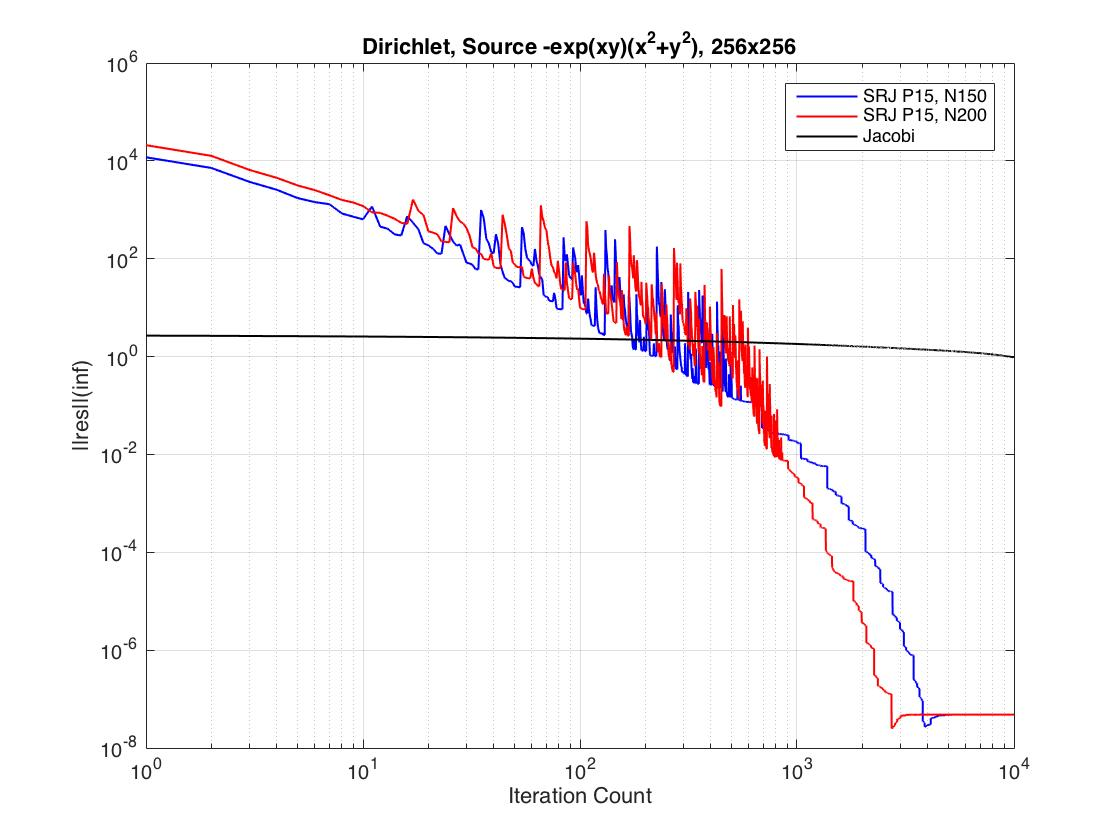
\includegraphics[scale=0.2]{exp(xy).jpg}
    \small{Figure 1: Infinity norm of residual vs Iteration count for linear, Dirichlet boundary value problem.}
\end{center}


We further test SRJ coupled with Newton-Raphson on a nonlinear PDE
\begin{equation}
    \triangle u +gu^3 = f
\end{equation}
In Figure 2, each color represents a different iteration in Newton-Raphson scheme with a fixed number of iterations of SRJ.
\begin{center}
    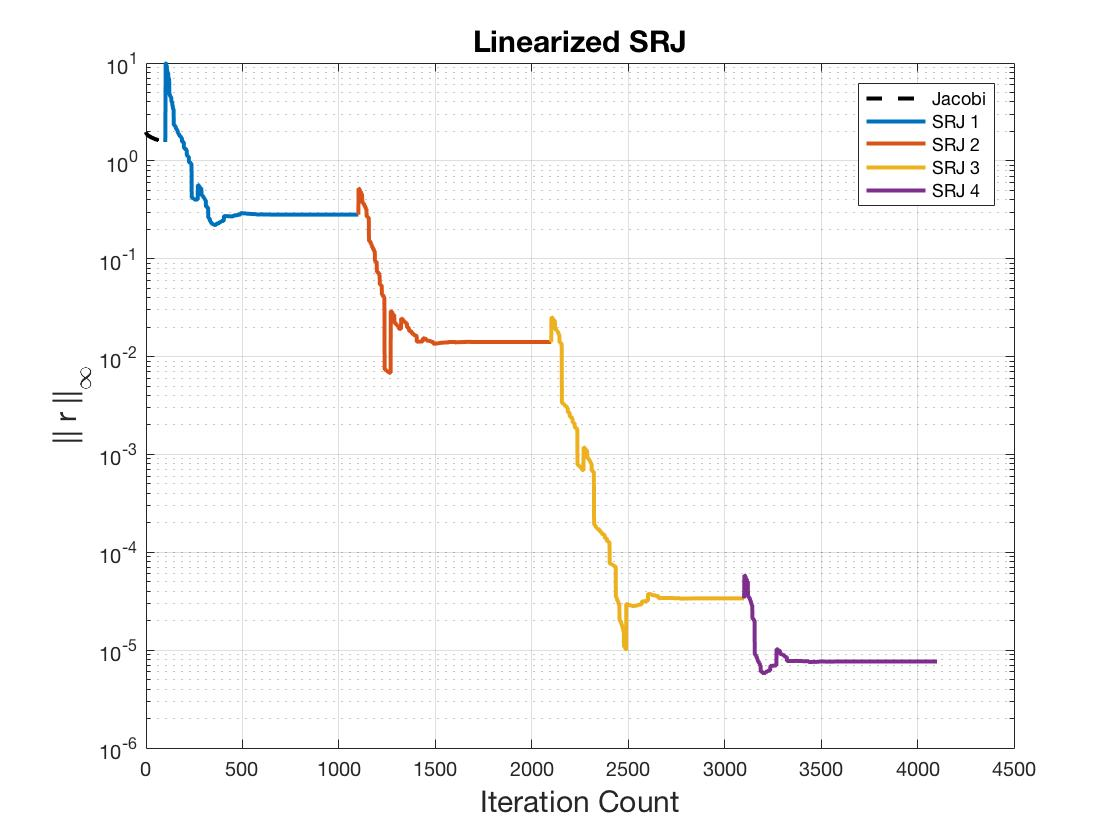
\includegraphics[scale=0.2]{SRJ.jpg} \\
    \small{Figure 2: Infinity norm of residual vs Iteration count for nonlinear, Dirichlet boundary value problem.}
\end{center}

We quantify the performance of our new method by computing initial data for the metric of a binary black hole system, and compare it to the solution obtained with TwoPunctures, a spectral solver in the Einstein Toolkit. Our solver converged to the solution produced by TwoPunctures within truncation error of our finite difference stencil.



\section{Preconditioned Krylov Subspace Methods}
Krylov Subspace Methods are a class of iterative solver for large, sparse linear systems. They work by forming a basis of the sequence of successive matrix powers times the initial residual. The approximation to the solution is then obtained by minimizing the residual over the basis formed. Hence, Krylov subspace methods are bound to converge in $N$ iterations where $N$ is the size of the system $Au=f.$ Moreover, for large $N$, the iterative process is likely to reach sufficient accuracy well before.

The convergence properties of Krylov subspace methods can be improved by employing a preconditioner. A preconditioner, $M$, is a lower order approximation to the inverse of a matrix $A$ such that $MA$ has a low condition number.In preconditioned Krylov subspace methods, we solve $M(Au-f)=0$.

\subsection{Preconditioner}
A suitable preconditioner is able to reduce the number of iterations by multiple orders of magnitude. We design a preconditioner that affectively treats the Laplacian, $\triangle\cdot$, the dominant term and major source of stiffness in initial data problems. Consider the two dimensional boundary value problem

\begin{align}
    \triangle u(\mathbf{x}) &= f(\mathbf{x}), \mathbf{x}\in\Omega \\
    u &= 0, \mathbf{x}\in\partial\Omega
\end{align}

where $\Omega$ is a domain of \mathbf{x}. We discretize $(5)$ using the standard five point finite difference stencil and $n$ points per dimension following the standard lexicographical ordering to obtain a system of algebraic equations:
\begin{equation}
    Mu = f
\end{equation}

The spectral decomposition of $M$ is known. For $k,l=1,2,...,n$, the eigenvectors and eigenvalues are
\begin{align}
    s_{kl} &= \sin{k\pi x}\sin{l\pi y} \\
    \lambda_{kl} &= -\dfrac{2}{h_x^2}(1-\cos{k\pi h_x}) -\dfrac{2}{h_y^2}(1-\cos{l\pi h_y})
\end{align}
where $h_x,h_y$ are grid spacing in $x$ and $y$ direction.
Diagonalizing $M$, we get
\begin{equation}
    M = S^\text{T} \Lambda S
\end{equation}
where $S$ the orthonormal matrix of column eigenvectors and $\Lambda$ is the diagonal matrix of eigenvalues. In this form, $M$ can be easily inverted as $\Lambda$ is diagonal.
\begin{equation}
    M^{-1} = S^\text{T}\Lambda^{-1}S
\end{equation}
We use $M^{-1}$ as our preconditioner. We further reduce the computatinoal cost of applying $M^{-1}$ to a vector from $\mathcal{O}(N^2)$ to $\mathcal{O}(N\log N)$ by realizing that matrix vector products with $S$ of a vector $v$ is equivalent to taking a discrete sine transform of $v$.

\subsection{Implementation}
We implement preconditioned Krylov subspace methods using two numerical libraries in C, PETSc (Portable, Extensible Toolkit for Scientific Computation) and FFTW (Fast Fourier Transform in the West). We use Biconjugate Gradient Stabilized (BiCG) scheme from PETSc as BiCG is able to handle non symmetric matrices. FFTW contains discrete sine transforms.

Our implementation is matrix-free in order to avoid the large cost associated with storing $N^2$ floating point values. As a result, all matrix vector products cost $\mathcal{O}(N).$

\subsection{Results}
We restrict ourselves to showing results for linear equations as we have already demonstrated the Newton-Raphson scheme that handles nonlineaerities. Figure 3 contains plot of residual vs number of iterations for the Dirichlet boundary value problem (3) discretized using the standard five-point finite difference stencil with 500 grid points in each direction. The residual decreases by an order of magnitude at every iteration of preconditioned BiCG until it reaches truncation error in ~10 iterations.

\begin{center}
    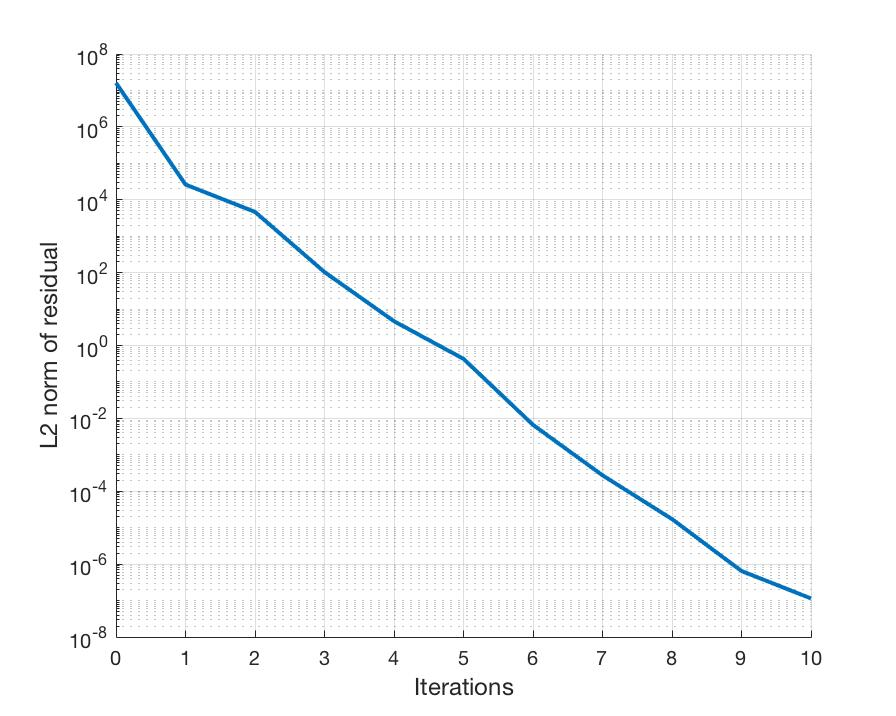
\includegraphics[scale=0.25]{res.jpg} \\
    \small{Figure 3: Infinity norm of residual vs Iteration count for linear, Dirichlet boundary value problem.}
\end{center}

A major drawback of relaxation schemes and Krylov subspace methods is that the number of iterations depend on the size of the system to be solved. We test our method on equation $(3)$ with grid sizes varying from 50 by 50 to 2000 by 2000. From figure 4, we can see that the number of iterations until truncation error is reached is roughly constant for a wide range of grid sizes.

\begin{center}
    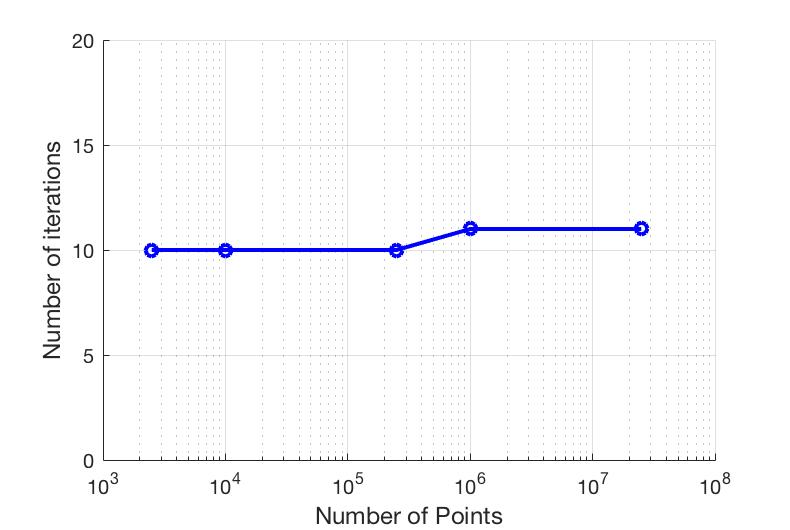
\includegraphics[scale=0.3]{iterations.jpg} \\
    \small{Figure 4: Iterations to truncation error vs Grid size for linear, Dirichlet boundary value problem.}
\end{center}

\section{Conclusion and Future Work}
We have two $\mathcal{O}(N)$ schemes for solving nonlinear, Dirichlet boundary value problems on a single grid. We intend to do a literature search on how the two schemes would behave as a smoothing operation of a multigrid solver. Additionally, we would need to modify the error equation in CT\_Multilevel accordingly.

\begin{thebibliography}{9}

\bibitem{1}

  Xiyang Yang, Rajat Mittal,
  \textit{Acceleration of the Jacobi iterative method by factors exceeding 100 using scheduled relaxation},
  Department of Mechanical Engineering, Johns Hopkins University,
  2014.
  \bibitem{2}
  J.~E.~Adsuara, I.~Cordero-Carrión, P.~Cerdá-Durán and M.~A.~Aloy,
  J.\ Comput.\ Phys.\  {\bf 321}, 369 (2016)
  doi:10.1016/j.jcp.2016.05.053
  [arXiv:1511.04292 [math.NA]].

\end{thebibliography}

\end{multicols}

\end{document}